\chapter{Geth共識模組程式架構與私有鏈系統部署}\label{se_5}
在5.1將會介紹我們如何修改Geth(以太坊go語言版本)的共識模組,並且介紹共識模組彼此關係。5.2將會介紹如何將修改後的共識模組放到雲端平台上並有效率的讓這些雲端平台上的機器組成私有鏈。
\section{Geth共識模組程式架構}\label{se_5}
本章節介紹我們如何實作拜占庭容錯共識的架構。我們的程式架構主要參考NCCU-BFT \cite{nccubft}與MSIG-BFT \cite{chen2018msig}。共識模組底下包含處理訊息的 Message Handler、同步訊息的 Synchronizer、與三個主要做共識的模組,Consensus Manager、Height Manager與Round Manager。共識模組間的關係如圖5.1。
各共識模組之間相互負責不同事情。共識模組透過go語言來進行實作,模組間參數時常共同管理(透過 go語言裡Channels來傳遞參數),因此需要透過讀寫鎖來控制讀寫流程,才不會造成多個模組同時讀寫情形。
節點間訊息傳輸前都需透過橢圓數位簽名演算法進行簽名(ECDSA) \cite{ecdsa},以確保訊息沒有被竄改。  

\begin{figure}[h]
\centering
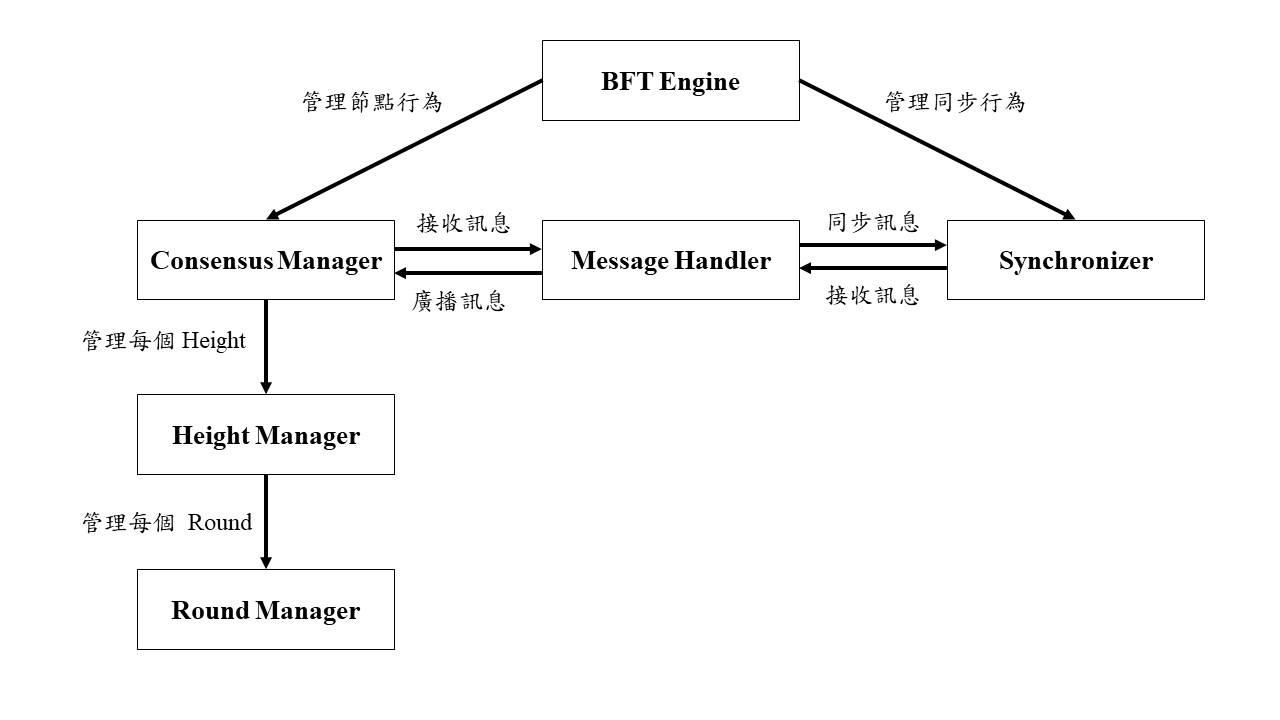
\includegraphics[scale=0.45]{images/5.jpg}
\caption{共識模組關係圖。}
\label{i:byz-latency}
\end{figure}

\newpage

\subsection{Consensus Manager}\label{se_5} 
Consensus Manager主要管理節點間連線,並且紀錄參與共識時所需的各式資訊,如:私有鏈ID、各節點地址、共識Timeout等。
並且檢查區塊內的交易是否合法。Consensus Manager 核心技術在於定時的檢查自身狀態是否符合下列三點。(一)廣播:檢查是否為該回合的廣播提議者,如果是則打包資料庫裡交易紀錄提出Proposal;如果不是則等待Proposal被提出。(二)投票:檢查是否有收到Proposal,如果有則檢查是否合法;如果沒收到則對上回合的提議再次投票。(三)提交:檢查票集合是否有足夠票數的票據,如果有則提交區塊。如果滿足上述任何一個狀態,則透過呼叫下層 Height Manager,進一步處理共識。同時也要將需要廣播的資訊交給 Message Handler進行廣播。
\subsection{Height Manager}\label{se_5}
此模組主要功能是處理某一個高度的共識,透過管理一或多個 Round Manager 與其他節點溝通。(一)廣播:如果節點為該回合的Proposer且擁有前一回合票集合,呼叫下層 Round Manager 廣播新的共識提議;如果節點不是此回合的Proposer,等待新的共識提議被提出。(二)投票:呼叫Round Manager幫忙進行投票。(三)提交:確認高度是否已達成共識,如果還沒則呼叫Round Manager進行提交共識。

\subsection{Round Manager}\label{se_5}
每個高度可能會需要一到多個回合,最終才能達成共識。因此Height Manager可能須要建立多個Round Manager來進行共識。Round Manager 會蒐集來自Height Manager的訊息(目前共識高度訊息),經過判斷後採取對應動作。(一)廣播:對所有節點廣播共識提案、(二)投票:在一個回合裡,Round Manager只會對一個合法共識提案簽章並廣播,因此Round Manager會檢查是否已經對某高度投過票。(三)提交:將區塊內容同步到自身資料庫,並進入下一個區塊高度。


\subsection{Message Handler}\label{se_5} 
Message handler 主要負責接收與廣播共識之中需要的訊息,在接收到來自其他節點的訊息時,進行判斷是否交給 Consensus Manager,或是過濾掉重複接受的訊息。

\subsection{Synchronizer}\label{se_5}
Synchronizer 主要目的為同步節點間狀態。因為網路間可能存在延遲或訊息也可能丟失,因此可能導致部分節點沒有收到新的共識提議而無法執行後續共識。這時候節點必透過Synchronizer先與其他節點索取必要資訊(例如:沒收到的共識提議)並且同步到最新狀態。  


\section{私有鏈系統部署}\label{se_5}  
TwoStepBFT共識演算法相較於過去傳統三回合的共識演算法,能在網路傳輸穩定情況下能較快達成共識。我們的目標是測試TwoStepBFT在多個節點的私有鏈效率,實驗將在AWS雲端伺服器上進行。因此,實驗目標將分為(一)雲端虛擬機器設定:依照使用者需求,在雲端平台上開啟多台規格一致的機器作為私有鏈節點。(二)私有鏈系統設定:將雲端平台上的機器依使用者設定參數客製化搭建私有鏈。為了達成上述兩項目標,我們整合了許多自動化的開發套件來協助我們完成實驗。實驗系統架構主要如下圖5.1所描述。
\begin{figure}[htbp]
\centering
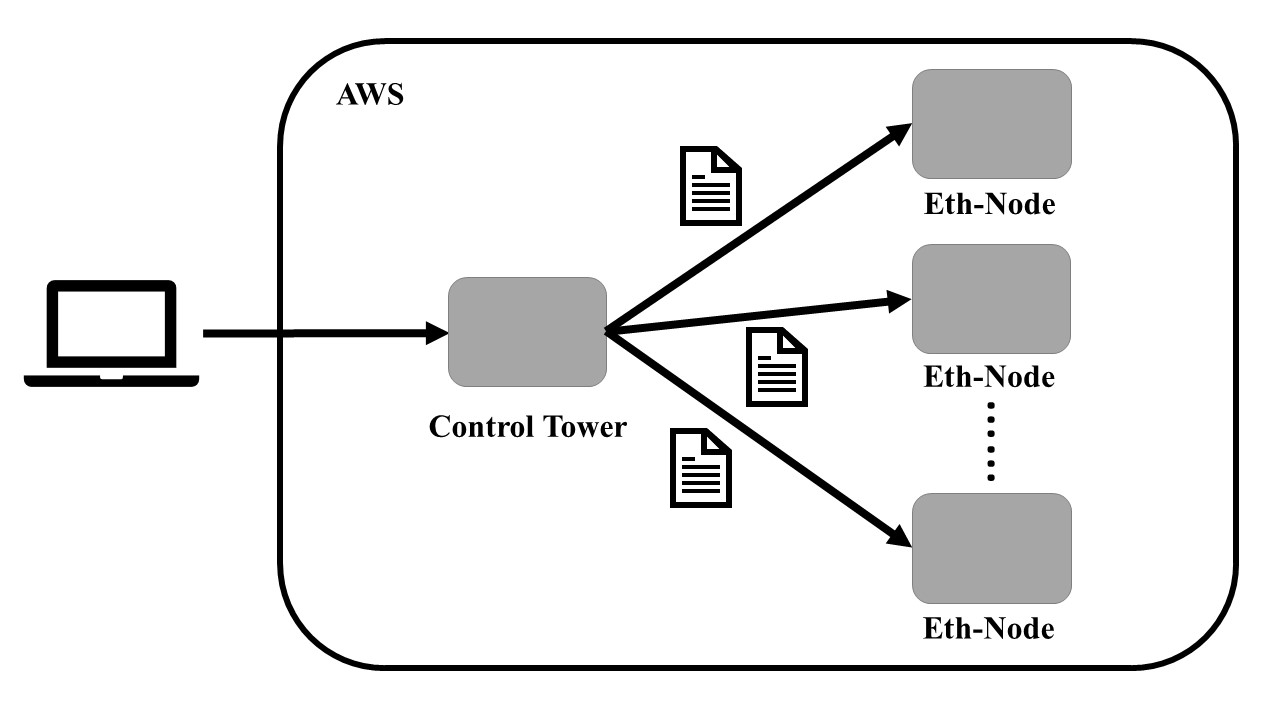
\includegraphics[scale=0.5]{images/51.jpg}
\caption{實驗系統架構圖。}
\label{i:byz-latency}
\end{figure}
該系統內含一個Control Tower,此台電腦類似實驗的中央控制中心,負責部署實驗環境到其他雲端機器上,並且收集其他機器所產生的實驗數據。依照不同需求,系統內包含數台規格一致機器作為區塊鏈節點,這些節點運行TwoStepBFT演算法以達成區塊鏈共識。

\subsection{雲端虛擬機器設定}\label{se_5} 
為了能夠在雲端平台上,快速開啟多台環境一致的機器,這些機器將成為區塊鏈的節點。我們的步驟為下(一)透過Packer將系統所需套件打包成映像檔。該映像檔裡需包含TwoStepBFT共識專案以及程式所需的各試工具套件,例如:Go語言套件、Node.js等套件,以便後續私有鏈搭建。
將所需套件打包成映像檔好處如下。
\begin{itemize}%项目符号开始

\item 快速的部署:映像檔內已包含所須套件,不需要逐一安裝套件,且也不怕遺漏安裝套件。

\item 跨平台且可攜性:不同平台打包出的映像檔,可以獲得相同的運行環境且這個映像檔能夠兼容不同作業系統。
\end{itemize}

(二)依照使用者需求,透過Terraform快速在雲端平台上開啟多台規格一致的機器,並將步驟一產生的映像檔植入這些機器。
Terraform能夠快速將AWS環境架設起來,依照使用者所撰寫程式碼搭建出所描述的架構,Terraform好處是能徹底實現基礎架構即代碼IaC (Infrastructure as code),利用代碼來配置實驗環境,讓環境安全且方便管理。
Terraform的優點如下。
\begin{itemize}%项目符号开始

\item 將基礎架構使用語法進行描述,可讓建構計劃像一般程式碼一樣進行版本控管與追蹤。 

\item Terraform會自動分析本地端計劃與遠端是否一至,自動化修改從而避免許多可能的人為操作錯誤。
\end{itemize}

\subsection{私有鏈系統設定}\label{se_5} 
此小節將會介紹如何將修改後的共識模組放到雲端平台上,並有效率的讓這些雲端平台上的機器搭建出一條私有鏈。
為了方便的控制雲端平台上的所有機器,我們使用Ansible來管理節點間的行為。Ansible能夠定義群組,一個群組裡能夠管理多個IP,透過此方法我們能為雲端平台上的機器定義出Control Tower與Eth-nodes。有了Ansible後,我們只需要操作Control Tower就能同時控制所有Eth-nodes,不需登入所有Eth-nodes機器進行操作。Ansible的優點如下。
\begin{itemize}%项目符号开始
\item 輕量級套件,無需在客戶端安裝agent,更新時,只需在操作機上進行一次更新即可。

\item 可將任務寫成腳本批次執行。

\item 使用python編寫,維護更簡單 。
\end{itemize}
Go-ethereum搭建私有鏈大致分為以下步驟(一)創建節點帳號(二)搭建私有鏈節點(三)連接各節點,下面說明各步驟。

(一)創建節點帳號:透過Control Tower命令Eth-nodes產生節點帳號資訊,在我們的實驗裡是透過Ethereum Wallet api產生節點資訊(公私鑰、節點地址等等),並將各節點產生的節點地址回傳Control Tower,待後續初始化私有鏈使用。

(二)搭建私有鏈節點:依照使用者需求創造出Genesis.json。Genesis.json裡記錄了此私有鏈網路的所有初始條件。我們將Control Tower收集的節點地址寫入Genesis.json,用來分配初始節點資產。透過定義Genesis.json裡的GasLimit來制定私有鏈區塊大小。Genesis.json上還包含許多資訊,例如:私有鏈ID、挖礦難度等等。因應使用者需求,Genesis.json被設計成依照使用者需求動態產生,以方便實驗進行。Control Tower會將Genesis.json回傳給Eth-nodes,讓Eth-nodes產生符合私有鏈的節點。

(三)連接各節點:將各節點產生的節點ID回傳給Control Tower整合出Static-node.json,並發送回給所有節點。節點連線時會優先訪問Static-node.json進行連線,此目的是為了讓P2P網路成為完全圖(Complete graph),讓任兩節點間皆存在P2P連線。

\begin{figure}[H]
\centering
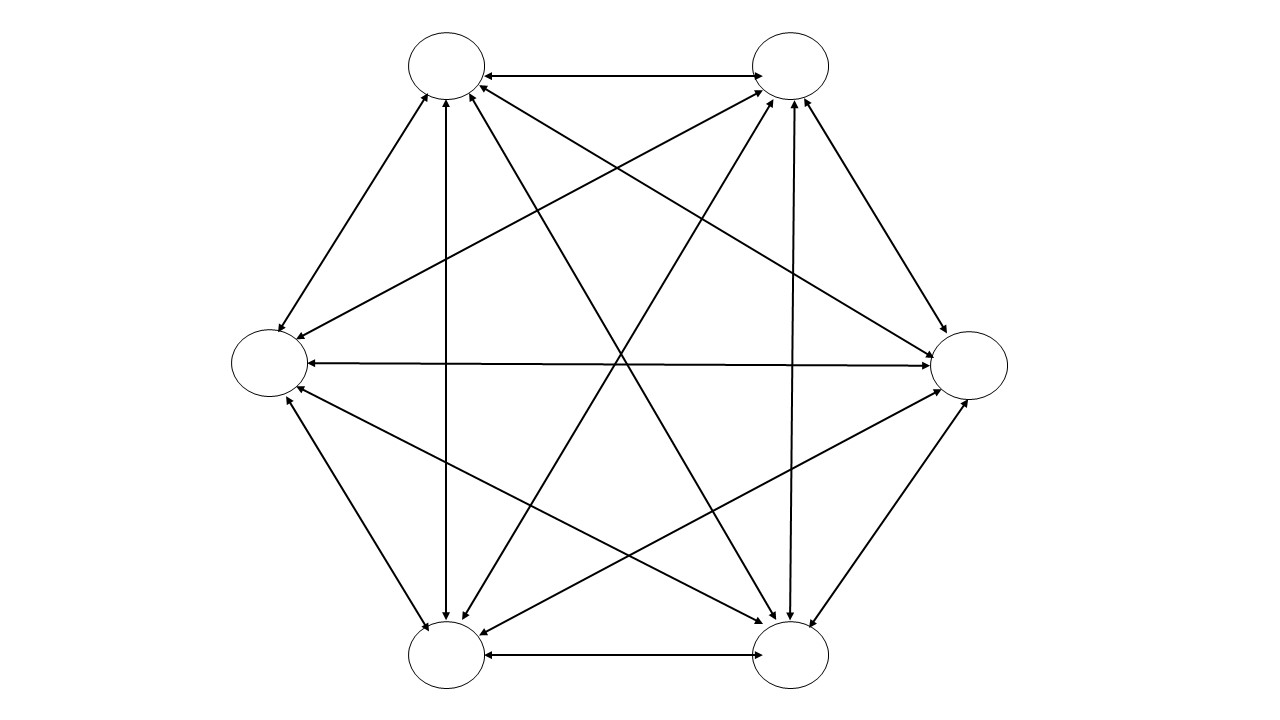
\includegraphics[scale=0.25]{images/6.jpg}
\caption{網狀連線範例圖。}
\label{i:byz-latency}
\end{figure}


 

%\item [3)]Eth-client: 在Eth-client裡我們會執行節點間相互交易,Eth-client幫助我們每秒產生數百筆交易,鏈上的節點才能打包這些交易成為候選區塊,故與Genesis.json 相同因每次實驗所產生節點帳戶地址都不相同,我們也將Eth-client設計成自動化動態產生。 

